\documentclass[10pt,aspectratio=169]{beamer}
\usetheme{Goettingen}
\usecolortheme{seahorse}

\usepackage{amsmath,amssymb}
\usepackage{graphicx}
\usepackage{booktabs}
\usepackage{algorithm}
\usepackage{algpseudocode}

\graphicspath{{../results/figures/}}

\title[Project 2]{Project 2}
\subtitle{Metaheuristic Optimisation of TSP Using Genetic Algorithm with Repair Mechanisms}
\author[]{Mutiara Jassy Atikah (P169188)\\Nur Ira Natasha Jafarizal (P168943)\\Muhamad Ridzuan Mohd Yazid Goi (P172103)}
\institute{Faculty of Information Science and Technology\\Universiti Kebangsaan Malaysia}
\date{June 2026}

\begin{document}

\begin{frame}[plain]
\titlepage
\end{frame}

\begin{frame}{Outline}
\tableofcontents
\end{frame}

%=============================================================================
\section{Problem}
%=============================================================================

\begin{frame}{kroA100 Benchmark}
\begin{columns}
\begin{column}{0.55\textwidth}
\begin{itemize}
    \item 100 cities, symmetric Euclidean distances
    \item Known optimal tour length: \textbf{21,282}
    \item Search space: $\sim 4.7 \times 10^{155}$ distinct tours
    \item From TSPLIB (Reinelt, 1991)
\end{itemize}

\medskip

Objective:
\[
\min_\pi \; f(\pi) = \sum_{i=0}^{n-1} d\!\left(\pi_i,\, \pi_{(i+1)\bmod n}\right)
\]

where $\pi$ is a permutation of $\{0,1,\ldots,99\}$.
\end{column}
\begin{column}{0.42\textwidth}
    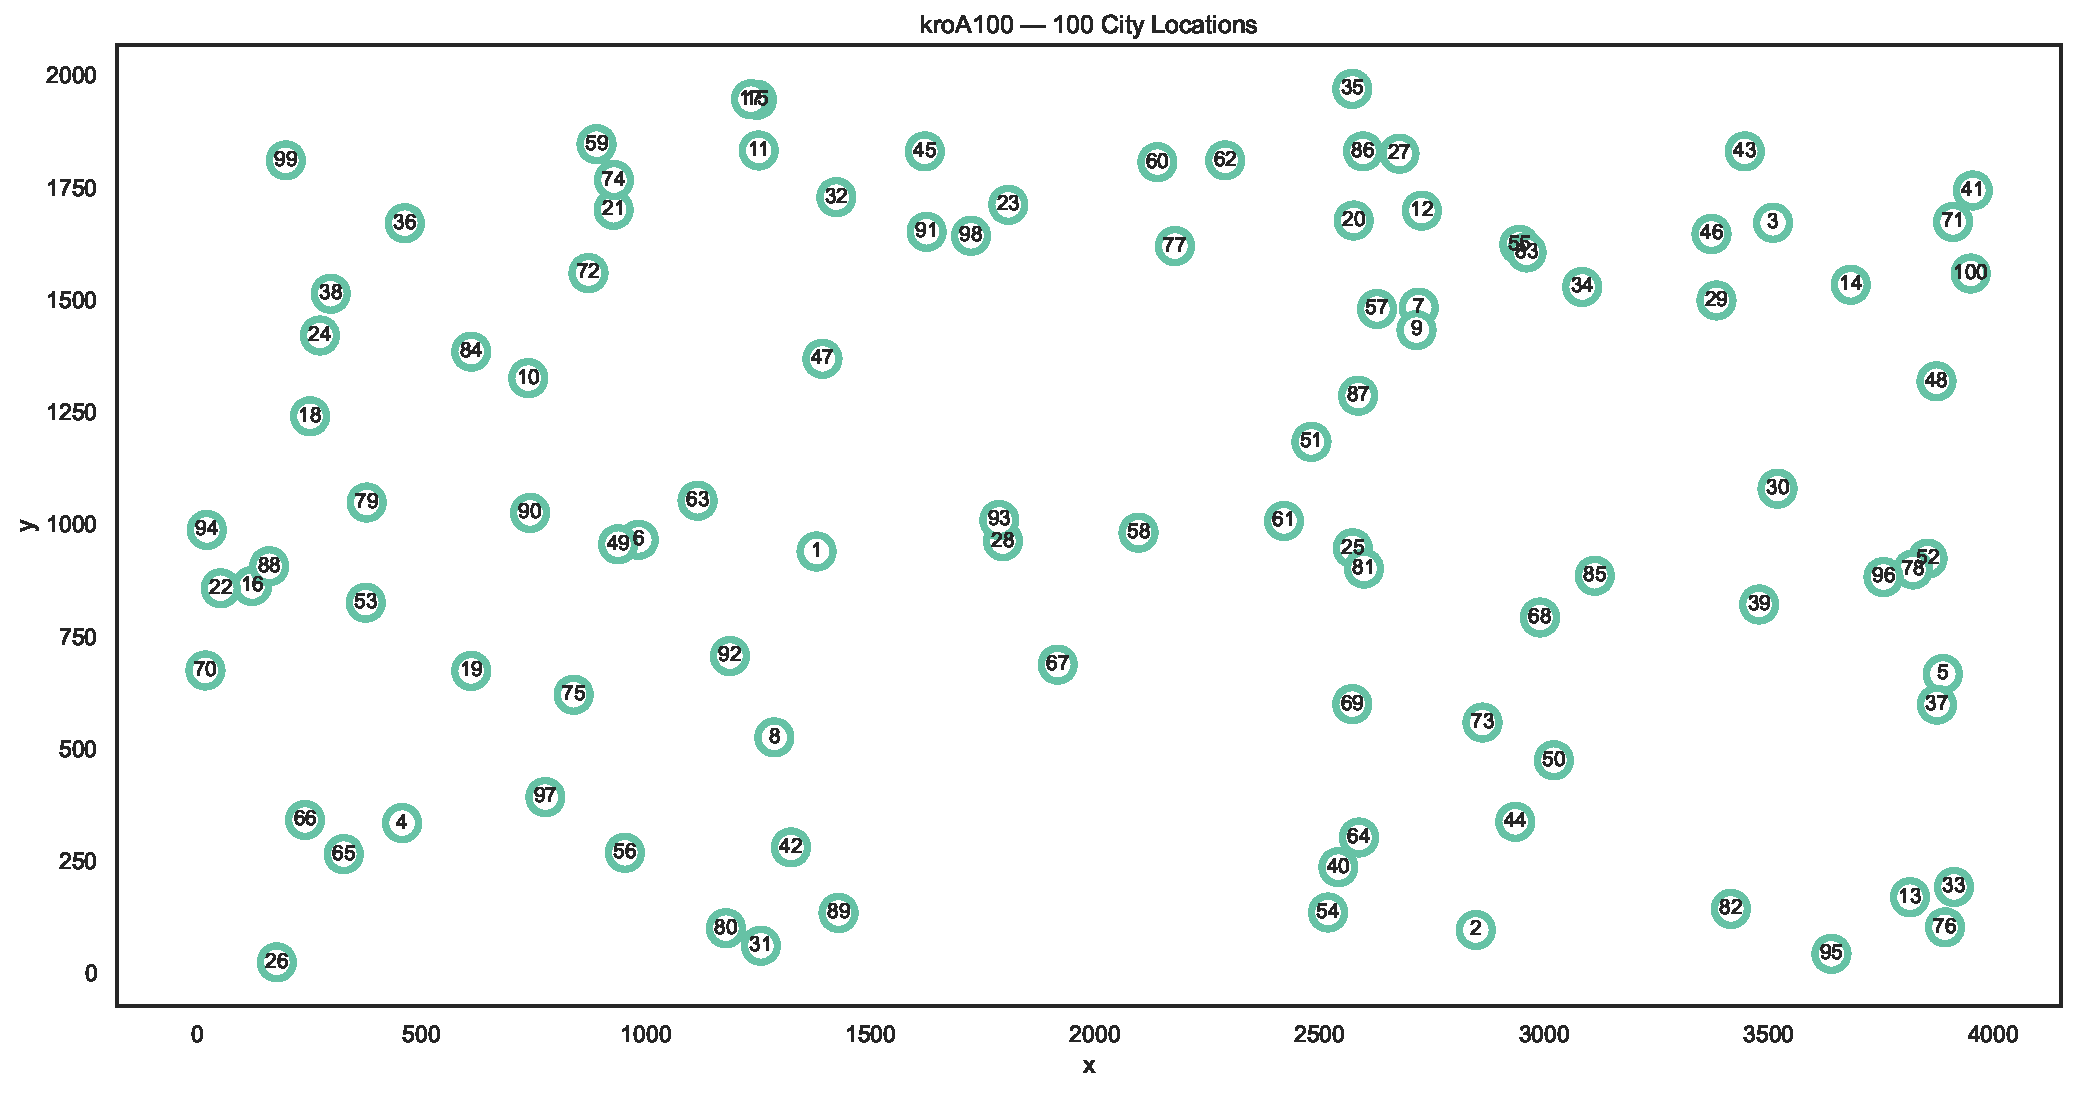
\includegraphics[width=\textwidth]{kroA100_cities.pdf}
\end{column}
\end{columns}
\end{frame}

%=============================================================================
\section{Genetic Algorithm}
%=============================================================================

\begin{frame}{Permutation Encoding}
\begin{itemize}
    \item Chromosome = ordered tuple of city indices
    \item Example (8 cities): $[3,0,7,1,5,2,6,4]$
    \item Tour: $3 \to 0 \to 7 \to 1 \to 5 \to 2 \to 6 \to 4 \to 3$
    \item Fitness = total closed tour length (lower is better)
\end{itemize}

\medskip

\begin{alertblock}{Permutation Constraint}
Every city must appear exactly once. A chromosome with duplicates or
missing cities is \textbf{not} a valid tour, even though the fitness
function still returns a number.
\end{alertblock}
\end{frame}

\begin{frame}{Evolutionary Operators}
\begin{columns}
\begin{column}{0.48\textwidth}
\textbf{Selection}
\begin{itemize}
    \item Tournament ($k{=}3$) -- primary
    \item Roulette wheel -- comparison
\end{itemize}

\medskip

\textbf{Crossover}
\begin{itemize}
    \item Naive single-point -- primary
    \item PMX -- feasibility-preserving comparison
\end{itemize}
\end{column}
\begin{column}{0.48\textwidth}
\textbf{Mutation}
\begin{itemize}
    \item Swap mutation -- sole operator
    \item Preserves permutation by construction
\end{itemize}

\medskip

\textbf{Other settings}
\begin{itemize}
    \item Elitism: top 2 carried over
    \item 500 generations, 30 seeds per config
    \item Pop size 200, $r_c{=}0.95$, $r_m{=}0.10$
\end{itemize}
\end{column}
\end{columns}
\end{frame}

\begin{frame}{Main Loop}
\footnotesize
\begin{algorithmic}[1]
\State Initialise population $P$ of $N$ random permutations
\State Evaluate fitness $f(p)$ for all $p \in P$
\For{$g = 1$ to $G_{\max}$}
    \State $P' \gets$ top-$e$ elites from $P$ \Comment{elitism}
    \While{$|P'| < N$}
        \State Select parents $p_1, p_2$ via tournament or roulette
        \If{$\mathrm{rand}() < r_c$}
            \State $c \gets \mathrm{Crossover}(p_1, p_2)$
        \Else
            \State $c \gets \mathrm{copy}(p_1)$
        \EndIf
        \State $c \gets \mathrm{Mutate}(c, r_m)$ \Comment{swap}
        \If{repair enabled}
            \State $c \gets \mathrm{Repair}(c)$
        \EndIf
        \State Append $c$ to $P'$
    \EndWhile
    \State $P \gets P'$; evaluate fitness for all $p \in P$
\EndFor
\State \Return best individual in $P$
\end{algorithmic}

\medskip
\normalsize
Lines 8 and 14 are the focus of this presentation: what goes wrong at
crossover, and how repair fixes it.
\end{frame}

%=============================================================================
\section{Constraint Handling}
%=============================================================================

\begin{frame}{Naive Crossover Breaks the Permutation}
\begin{center}
    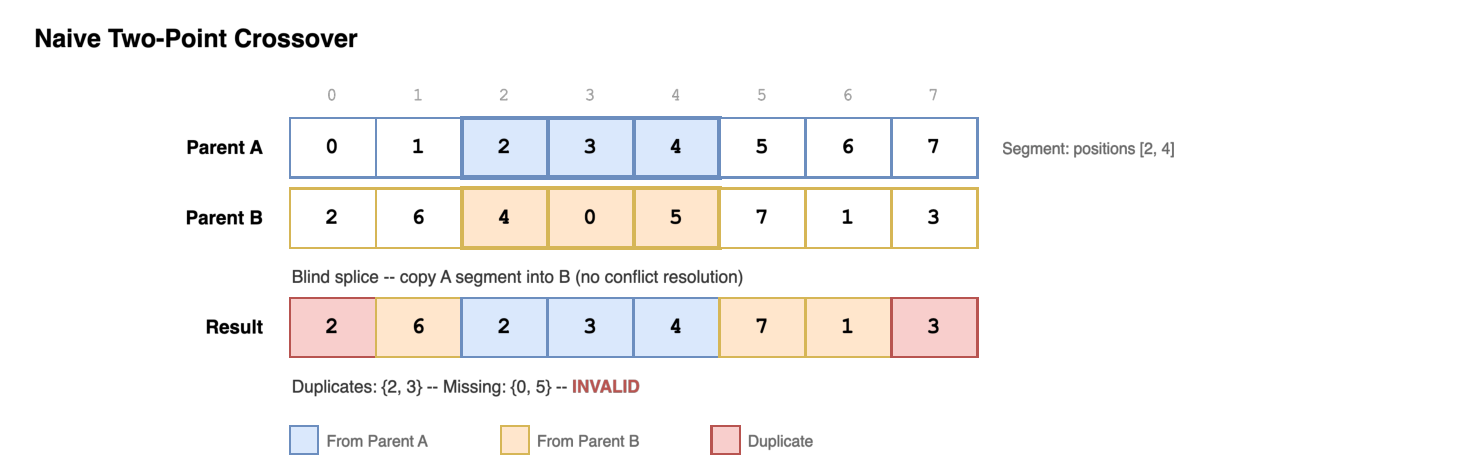
\includegraphics[width=0.82\textwidth]{naive_crossover.pdf}
\end{center}

Cities \{2, 3\} duplicated, cities \{0, 5\} missing.
The child is \textbf{not} a valid tour -- but the fitness function still
returns a number, and it tends to be artificially low.
\end{frame}

\begin{frame}{PMX Prevents It by Construction}
\begin{center}
    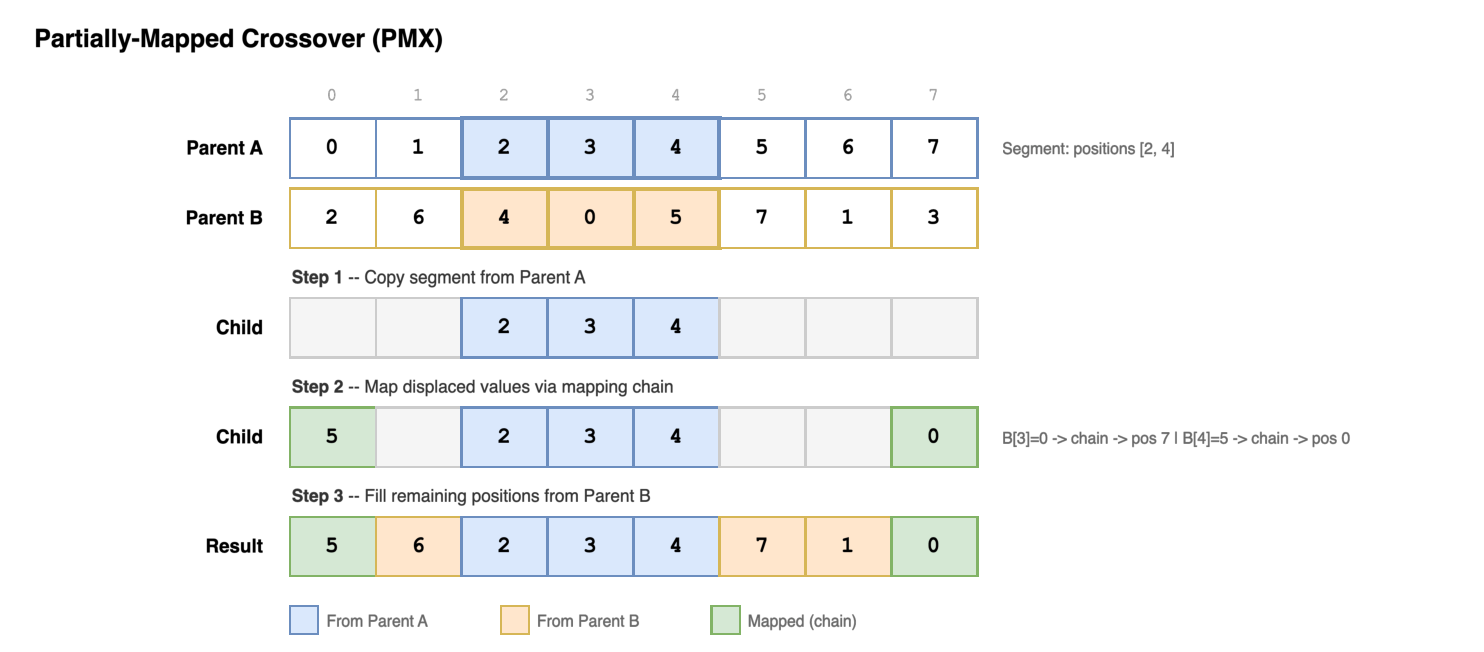
\includegraphics[width=0.82\textwidth]{pmx_crossover.pdf}
\end{center}

PMX copies the segment from Parent A, then routes displaced values through
a mapping chain until each lands in an unoccupied position.
Every city appears exactly once -- no repair needed.
\end{frame}

\begin{frame}{Our Approach: Repair After the Fact}
Instead of switching to PMX, we keep naive crossover and \textbf{repair}
every offspring. This makes repair load-bearing on every generation.

\medskip

\textbf{Phase 1 -- Diagnosis:} scan left to right, track \emph{seen} set,
flag duplicate positions, compute missing cities.

\medskip

\textbf{Phase 2 -- Correction} (random insertion):
shuffle missing cities, place at duplicate positions. No geometric bias,
preserves population diversity.

\medskip

\begin{example}
Input: $(3,1,4,\mathbf{1},5,2,6,\mathbf{3})$ \quad
Duplicates: $\{3,7\}$ \quad Missing: $\{0,7\}$\\
Random repair $\to$ $(3,1,4,\mathbf{7},5,2,6,\mathbf{0})$ \checkmark
\end{example}
\end{frame}

%=============================================================================
\section{Evaluation}
%=============================================================================

\begin{frame}{Experiment Setup}
Which strategy handles the permutation constraint best?
We run the same GA three ways on kroA100:

\bigskip

\begin{tabular}{ll}
\toprule
\textbf{Shared parameters} & pop=100, $r_c$=0.8, $r_m$=0.2, tournament, 500 gen \\
\textbf{Seeds} & 30 independent runs per strategy \\
\bottomrule
\end{tabular}

\bigskip

\begin{description}
    \item[Repair] Naive crossover + random-insertion repair.
          Every evaluated chromosome is a valid tour.
    \item[Penalty] Naive crossover, no repair. Infeasible offspring
          penalised by $w \cdot v$ ($w{=}50{,}000$) added to fitness.
    \item[PMX] Feasibility-preserving crossover. No repair needed.
\end{description}
\end{frame}

\begin{frame}{Results}
\begin{columns}
\begin{column}{0.48\textwidth}
\centering
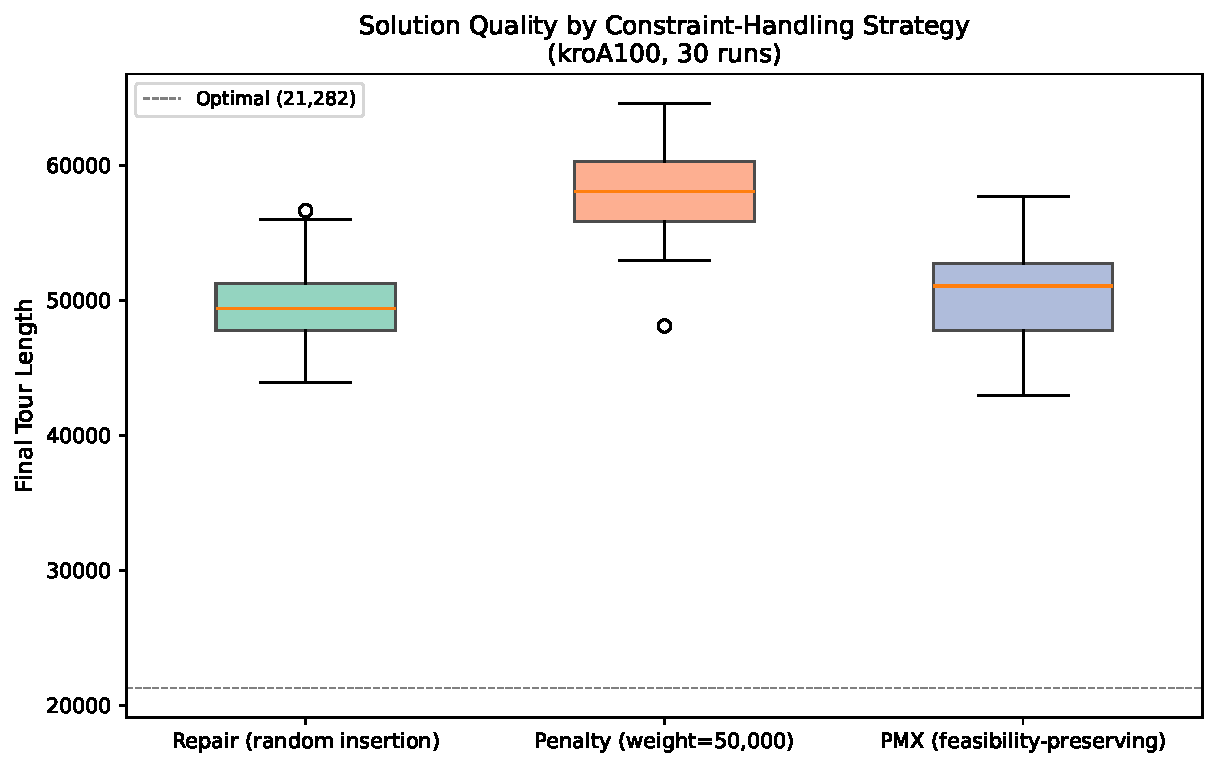
\includegraphics[width=\textwidth]{boxplot_strategy.pdf}
\end{column}
\begin{column}{0.48\textwidth}
\centering
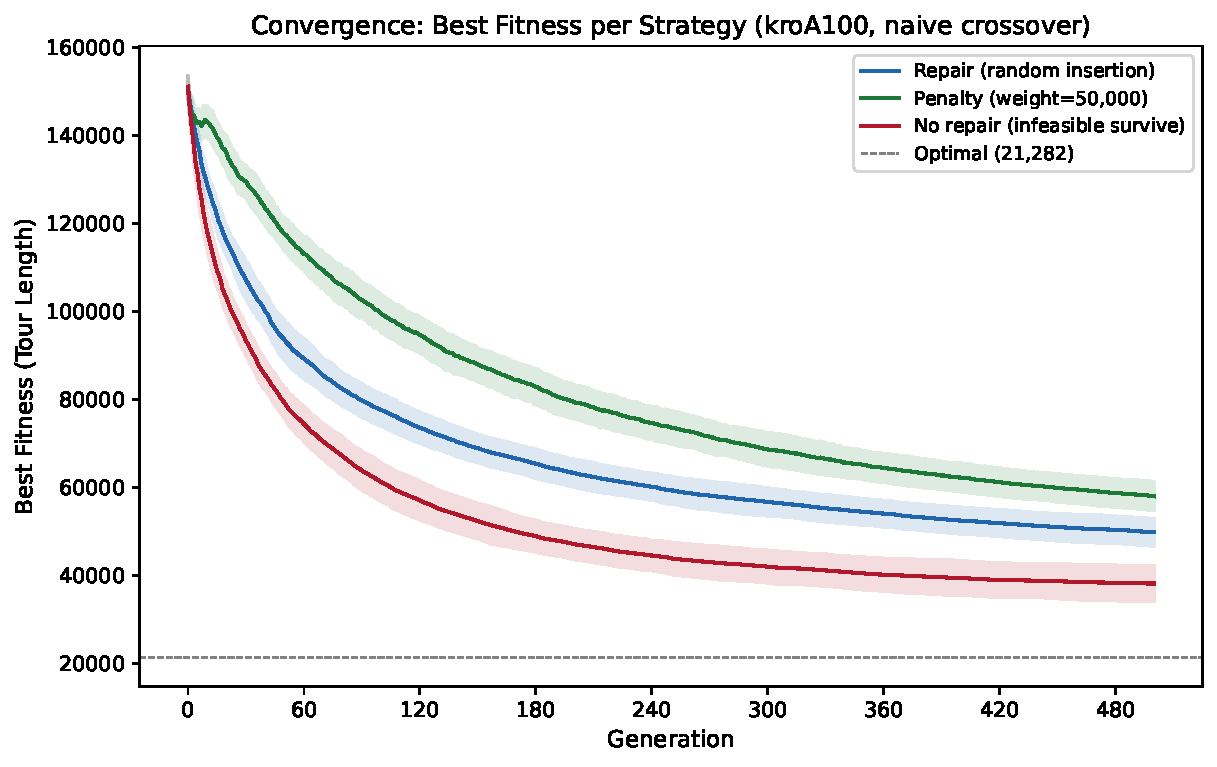
\includegraphics[width=\textwidth]{convergence_best_fitness.pdf}
\end{column}
\end{columns}

\medskip

\begin{tabular}{lrrr}
\toprule
Strategy & Mean best & Std & Gap \\
\midrule
Repair  & 49,778 & 3,187 & 133.9\% \\
PMX     & 50,655 & 3,573 & 138.0\% \\
Penalty & 57,948 & 3,285 & 172.3\% \\
\bottomrule
\end{tabular}

\smallskip
Repair and PMX are practically tied; penalty trails by ${\sim}16\%$.
\end{frame}

\begin{frame}{Takeaways}
\begin{enumerate}
    \item Naive crossover + repair is competitive with PMX on kroA100
          (mean gap differs by ${\sim}2\%$)
    \item Random insertion preserves diversity better than deterministic
          repair strategies
    \item Penalty function trails both feasibility-based approaches
          by ${\sim}16\%$
    \item Enforcing feasibility directly gives the GA a cleaner search
          signal than penalising infeasibility
\end{enumerate}

\bigskip
\centering
\Large Thank you
\end{frame}

\end{document}
